\documentclass{beamer}

\setbeamertemplate{footline}[frame number]

\usepackage{tikz}
\usepackage{centernot}
\usepackage[T1]{fontenc}


\title{Programmation système}
\author{Processus, threads, goroutines}
\date{loig.jezequel@univ-nantes.fr}

\begin{document}


\frame{
\maketitle
}

% on parle de prog concurrente
% pourquoi ?
% exemples : 
% - accès lent à une ressource (disque, utilisateur), ne pas laisser le processeur en pause
% - plusieurs choses à la fois "simplement"
% concurrent vs. parallèle

\frame{
\frametitle{Concurrence}

\begin{center}
    Étant donné un ensemble d'évènements
  \end{center}

  \begin{block}{Il est dit {\bf sequentiel}}
    si tous ses évènements ont toujours lieu dans le même ordre
  \end{block}

  \uncover<2->{%
    \begin{block}{Il est dit {\bf concurrent}}
      si certains de ses évènements peuvent survenir dans différents ordres
    \end{block}%
  }

  \begin{center}
    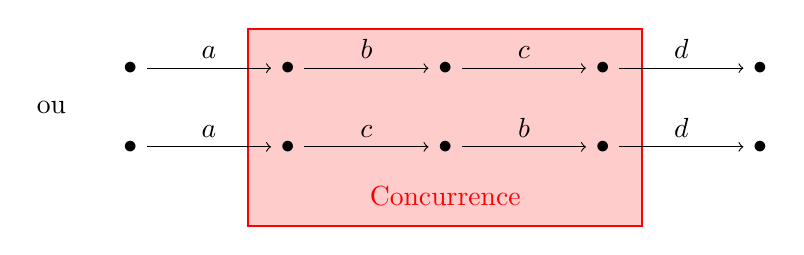
\begin{tikzpicture}[]
      \uncover<3>{%
        \draw[thick, red, fill=red!20] (1.5, 0.5) rectangle node[yshift=-25]{Concurrence} (6.5, -2);%
      }

      \node (0) at (0,0) {$\bullet$};
      \node (1) at (2,0) {$\bullet$};
      \node (2) at (4,0) {$\bullet$};
      \node (3) at (6,0) {$\bullet$};
      \node (4) at (8,0) {$\bullet$};

      \draw[->] (0) edge node[above]{$a$} (1);
      \draw[->] (1) edge node[above]{$b$} (2);
      \draw[->] (2) edge node[above]{$c$} (3);
      \draw[->] (3) edge node[above]{$d$} (4);

      \uncover<2->{%
        \node (0) at (0,-1) {$\bullet$};
        \node (1) at (2,-1) {$\bullet$};
        \node (2) at (4,-1) {$\bullet$};
        \node (3) at (6,-1) {$\bullet$};
        \node (4) at (8,-1) {$\bullet$};

        \draw[->] (0) edge node[above]{$a$} (1);
        \draw[->] (1) edge node[above]{$c$} (2);
        \draw[->] (2) edge node[above]{$b$} (3);
        \draw[->] (3) edge node[above]{$d$} (4);

        \node (info) at (-1,-0.5) {ou};%
      }
    \end{tikzpicture}
  \end{center}

}

\frame{
\frametitle{Importance de la concurrence en programmation système}

\begin{itemize}
\item Temps «long» pour accéder aux périphériques
\begin{itemize}
\item quelques millisecondes pour accéder à des données sur un disque dur
\item quelques milliards d'opérations par seconde pour un processeur
\end{itemize}
\item Temps «très long» et imprévisible pour les interactions de l'utilisateur
\item Exécution séquentielle des tâches non souhaitable
\end{itemize}

}

\frame{
  \frametitle{Concurrence ou parallélisme ?}

  \begin{block}{Concurrence}
    On ne sait pas dans quel ordre des évènements concurrents se déroulent
  \end{block}

  \begin{block}{Parallélisme}
    Des évènements parallèles peuvent se dérouler en même temps
  \end{block}

  \begin{alertblock}{Parallélisme $\implies$ concurrence}
    Des évènements parallèles sont aussi concurrents
  \end{alertblock}

  \pause

  \begin{alertblock}{Concurrence $\centernot\implies$ parallélisme}
    On peut exécuter des évènements concurrents sur une architecture ne permettant pas le parallélisme, mais des évènements concurrents \textcolor{red}{\bf se parallélisent naturellement}.
  \end{alertblock}

}

% la solution classique = processus
% quelques commandes sur les processus (top, ps, kill — remarque sur les signaux ?)

\frame{
\centering
\Huge
Processus
}

{
\setbeamertemplate{footline}{D'après S. Faucou \hfill \insertpagenumber\,/\,\inserttotalframenumber}

\begin{frame}{Processus}

  \begin{definition}[Processus]
    On appelle \alert{processus} l'ensemble des activités résultant de l'exécution d'un programme au sein d'un système informatique

    Un processus encapsule:
    \begin{itemize}
      \item un flot de contrôle logique: donne l'illusion d'un accès permanent et exclusif à l'UC
      \item un espace d'adressage virtuel: donne l'illusion d'un accès complet et exclusif à la mémoire
    \end{itemize}

  \end{definition}

  Un processus peut être vu comme une coquille d'exécution associée à un programme.
\end{frame}

\begin{frame}{Processus concurrents}

  Lorsque plusieurs processus sont actifs simultanément, le noyau entrelace leurs exécutions.
  Le flot de contrôle logique masque cet entrelacement.

  \begin{center}
    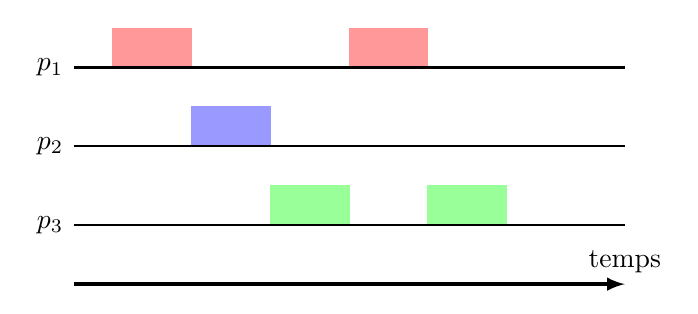
\begin{tikzpicture}
      % \draw[very thin, gray, step=.5cm] (0,0) grid (8,4);
      \draw[draw=red!40,fill=red!40] (1,3.5) rectangle (2,4);
      \draw[draw=red!40,fill=red!40] (4,3.5) rectangle (5,4);
      \draw[thick, black] (0.5,3.5) node [left] (p1) {$p_1$} -- (7.5,3.5) ;

      \draw[draw=blue!40,fill=blue!40] (2,2.5) rectangle (3,3);
      \draw[thick, black] (0.5,2.5) node [left] (p2) {$p_2$} -- (7.5,2.5) ;

      \draw[draw=green!40,fill=green!40] (3,1.5) rectangle (4,2);
      \draw[draw=green!40,fill=green!40] (5,1.5) rectangle (6,2);
      \draw[thick, black] (0.5,1.5) node [left] (p3) {$p_3$} -- (7.5,1.5) ;

      \draw[-latex, very thick, black] (0.5,0.75) -- (7.5,0.75) node [left, above] (legend) {temps} ;
    \end{tikzpicture}
  \end{center}

  Deux processus actifs simultanément sont \alert{en concurrence} pour accéder aux ressources de la machine.

\end{frame}

\begin{frame}{Exécution de processus concurrents}

  Ce que voit l'utilisateur : tous les processus s'exécutent en parallèle

  \begin{center}
    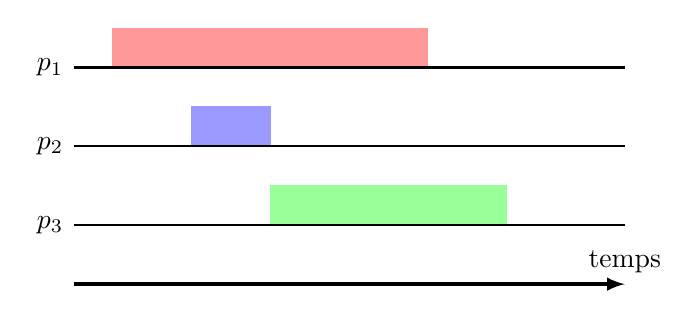
\begin{tikzpicture}
      \draw[draw=red!40,fill=red!40] (1,3.5) rectangle (5,4);
      \draw[thick, black] (0.5,3.5) node [left] (p1) {$p_1$} -- (7.5,3.5) ;

      \draw[draw=blue!40,fill=blue!40] (2,2.5) rectangle (3,3);
      \draw[thick, black] (0.5,2.5) node [left] (p2) {$p_2$} -- (7.5,2.5) ;

      \draw[draw=green!40,fill=green!40] (3,1.5) rectangle (6,2);
      \draw[thick, black] (0.5,1.5) node [left] (p3) {$p_3$} -- (7.5,1.5) ;

      \draw[-latex, very thick, black] (0.5,0.75) -- (7.5,0.75) node [left, above] (legend) {temps} ;
    \end{tikzpicture}
  \end{center}

  Ce qui se passe en réalité : le processeur est attribué par courtes tranches de temps aux processus concurrents

  \begin{center}
    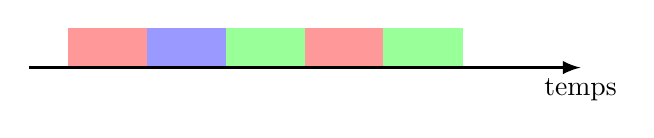
\begin{tikzpicture}
      \draw[draw=red!40,fill=red!40] (1,0.5) rectangle (2,1);
      \draw[draw=red!40,fill=red!40] (4,0.5) rectangle (5,1);
      \draw[draw=blue!40,fill=blue!40] (2,0.5) rectangle (3,1);
      \draw[draw=green!40,fill=green!40] (3,0.5) rectangle (4,1);
      \draw[draw=green!40,fill=green!40] (5,0.5) rectangle (6,1);
      \draw[-latex, very thick, black] (0.5,0.5) -- (7.5,0.5) node [left, below] (legend) {temps} ;
    \end{tikzpicture}
  \end{center}


\end{frame}

\begin{frame}{Changement de contexte (context switch)}
  Pour donner l'impression de simultanéité, le SE change très régulièrement le processus en cours :
  \begin{itemize}
    \item sauvegarde l'état du processus préempté (processeur $\rightarrow$ mémoire)
    \item charge de l'état du processus élu (mémoire $\rightarrow$ processeur)
  \end{itemize}

  \begin{center}
    \scalebox{0.9}{
      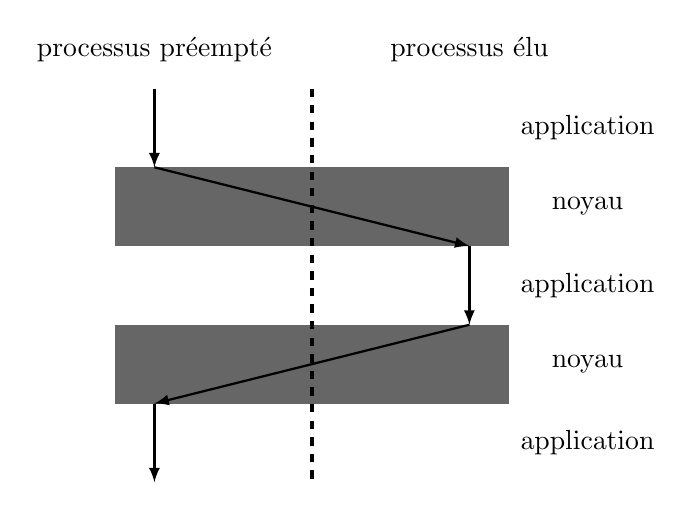
\begin{tikzpicture}
        \fill[black!60] (2.5,4) rectangle (7.5,3);
        \fill[black!60] (2.5,2) rectangle (7.5,1);
        \draw[dashed, very thick] (5,5) -- (5,0);
        \node (u1) at (8.5,4.5) {application};
        \node (u1) at (8.5,3.5) {noyau};
        \node (u1) at (8.5,2.5) {application};
        \node (u1) at (8.5,1.5) {noyau};
        \node (u1) at (8.5,0.5) {application};
        \node (proc1) at (3,5.5) {processus préempté};
        \node (proc1) at (7,5.5) {processus élu};
        % \draw[step=.5cm,gray,very thin] (0,0) grid (10,6);
        \draw[-latex,thick] (3,5) -- (3,4);
        \draw[-latex,thick] (3,4) -- (7,3);
        \draw[-latex,thick] (7,3) -- (7,2);
        \draw[-latex,thick] (7,2) -- (3,1);
        \draw[-latex,thick] (3,1) -- (3,0);
      \end{tikzpicture}}
  \end{center}
\end{frame}


\begin{frame}{Exécution de processus concurrents}

  Ce que voit l'utilisateur : tous les processus s'exécutent en parallèle

  \begin{center}
    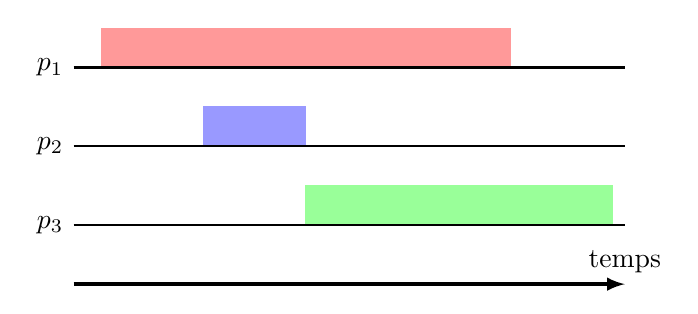
\begin{tikzpicture}
      % \draw[very thin, gray, step=.5cm] (0,0) grid (8,4);
      \draw[draw=red!40,fill=red!40] (0.85,3.5) rectangle (6.05,4);
      \draw[thick, black] (0.5,3.5) node [left] (p1) {$p_1$} -- (7.5,3.5) ;

      \draw[draw=blue!40,fill=blue!40] (2.15,2.5) rectangle (3.45,3);
      \draw[thick, black] (0.5,2.5) node [left] (p2) {$p_2$} -- (7.5,2.5) ;

      \draw[draw=green!40,fill=green!40] (3.45,1.5) rectangle (7.35,2);
      \draw[thick, black] (0.5,1.5) node [left] (p3) {$p_3$} -- (7.5,1.5) ;

      \draw[-latex, very thick, black] (0.5,0.75) -- (7.5,0.75) node [left, above] (legend) {temps} ;
    \end{tikzpicture}
  \end{center}

  Ce qui se passe en réalité : le noyau effectue régulièrement des changements de contexte.

  \begin{center}
    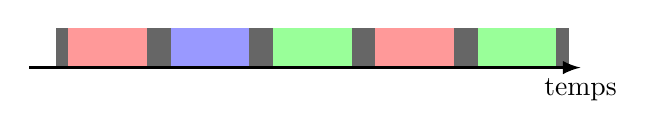
\begin{tikzpicture}
      \draw[draw=black!60,fill=black!60] (0.85,1) rectangle (1, 0.5);
      \draw[draw=red!40,fill=red!40] (1,0.5) rectangle (2,1);
      \draw[draw=black!60,fill=black!60] (2,1) rectangle (2.3, 0.5);
      \draw[draw=blue!40,fill=blue!40] (2.3,0.5) rectangle (3.3,1);
      \draw[draw=black!60,fill=black!60] (3.3,1) rectangle (3.6, 0.5);
      \draw[draw=green!40,fill=green!40] (3.6,0.5) rectangle (4.6,1);
      \draw[draw=black!60,fill=black!60] (4.6,1) rectangle (4.9, 0.5);
      \draw[draw=red!40,fill=red!40] (4.9,0.5) rectangle (5.9,1);
      \draw[draw=black!60,fill=black!60] (5.9,1) rectangle (6.2, 0.5);
      \draw[draw=green!40,fill=green!40] (6.2,0.5) rectangle (7.2,1);
      \draw[draw=black!60,fill=black!60] (7.2,1) rectangle (7.35, 0.5);
      \draw[-latex, very thick, black] (0.5,0.5) -- (7.5,0.5) node [left, below] (legend) {temps} ;
    \end{tikzpicture}
  \end{center}

\end{frame}

\begin{frame}{Contexte d'un processus}

  Le contexte d'un processus est constitué de l'ensemble des informations relatives aux processus stockées dans des ressources communes de la machine qui doivent être sauvegardées ou restaurées lors d'un changement de contexte :

  \begin{itemize}
    \item
      le pointeur d'instruction
    \item
      les pointeurs de pile et de cadre
    \item
      les registres
    \item
      quelques autres informations utiles au système
  \end{itemize}

  \bigskip

  Ces informations sont stockées dans une zone dédiée de la mémoire du noyau.
  Elles forment une partie du \alert{Process Control Block (PCB)}.

\end{frame}

}

\frame{
\frametitle{Organisation des processus}

\begin{block}{Caractéristiques d'un processus}
\begin{itemize}
\item Un PID (identifiant de processus)
\item Un parent (processus qui l'a créé)
\item Un état (en cours d'exécution, stoppé, terminé)
\end{itemize}
\end{block}

\begin{block}{Premier processus}
  Au démarrage, le noyau du système d'exploitation crée un processus d'initialisation.
\begin{itemize}
\item il porte le PID 1
\item il ne s'arrête jamais
\item il est la racine de l'arbre des processus
\item il adopte les processus orphelins
\end{itemize}
\end{block}

}

\frame{
\frametitle{Quelques commandes utiles sur les processus}

\begin{block}{ps}
Lister les processus
\end{block}

\begin{block}{top}
Voir \alert{dynamiquement} les processus qui s'exécutent, leur état, les ressources qu'ils consomment, etc
\end{block}

\begin{block}{kill}
Envoyer un \alert{signal} à un processus (par exemple pour lui demander de s'arrêter)
\end{block}

}

% des processus aux threads : entrées/sorties multiplexées
% les threads = mémoire partagée + changement de contexte plus léger + pas hiérarchie
% fils d'exécution au sein d'un processus, ordonnancés par l'OS

\frame{
\centering
\Huge
Threads
}

\frame{
\frametitle{Limitations des processus}

\begin{block}{Communication}
En l'absence de mémoire partagée, la communication entre processus est lourde à mettre en place.
\end{block}

\begin{block}{Contexte}
Le contexte d'un processus contient beaucoup d'informations ce qui rend coûteux~:
\begin{itemize}
\item la création de processus,
\item la destruction de processus,
\item le passage d'un processus à un autre (changement de contexte).
\end{itemize}
\end{block}

\begin{block}{Gestion}
La gestion assez rigide des processus implique fortement le système d'exploitation, notamment pour maintenir la structure arborescente qui doit exister entre eux.
\end{block}

}

\frame{
\frametitle{Threads (processus légers)}

\begin{itemize}
  \item Fils d'exécution séquentiels
\item Concurrents au sein d'un processus
\item Ordonnancés par le noyau du système d'exploitation
\item Mémoire partagée (entre threads d'un même processus)
\item Pile et registres privés
\item Changement de contexte peu coûteux
\item Pas de notion d'enfants/parents
\end{itemize}

}

% les goroutines
% mémoire partagée
% fils d'exécution au sein d'un processus, ordonnancés par le runtime Go (i.e. par le processus lui même)
% tout programme Go = plusieurs goroutines (ramasse miettes, main, etc)
% comment créer des goroutines volontairement
% quelques exemples de trucs qu'on peut faire avec les goroutines

\frame{
\centering
\Huge
Goroutines
}

\frame{
\frametitle{Goroutine}

\begin{itemize}
\item Fil d'exécution séquentiel
\item Plusieurs par thread (potentiellement)
\item Très léger ($10^6$ par processus)
\item Mémoire partagée (entre goroutines d'un programme)
\item API minimale (seule chose possible = démarrer une goroutine)
\item Ordonnancement par le scheduler du runtime Go
\end{itemize}

\vfill

\pause

\begin{block}{Par défaut}
main, ramasse miette
\end{block}

}

\frame{
\frametitle{Utiliser les goroutines}

\begin{block}{On utilise le mot clé go pour démarrer une goroutine}
ping-pong.go
\end{block}

\begin{block}{Main est plus importante que les autres}
main.go
\end{block}

\begin{block}{L'ordre d'exécution n'est pas controllable}
schedule.go
\end{block}

\begin{block}{La mémoire est partagée}
global.go\\
local.go
\end{block}

\begin{block}{On peut lancer beaucoup de goroutines en même temps}
many.go
\end{block}

}

\frame{
\frametitle{Ordonnancement, vu de loin}

\begin{block}{M:P:N Threading (en général, $N>M>P$)}
  \begin{itemize}
\item M threads,
\item P processeurs,
\item N goroutines.
\end{itemize}
Pour s'exécuter \alert{une goroutine est associée à un thread}, qui est lui-même \alert{associé à un processeur}.
\end{block}

\begin{block}{Choix des goroutines à exécuter}
\begin{itemize}
\item Une file d'attente par processeur
\item Points d'intérêt permettant un changement (appels de fonctions notamment)
\item Préemption pour assurer l'équité entre goroutines
\end{itemize}
\end{block}

}

\frame{
\frametitle{Pourquoi $M > P$ ?}

\begin{block}{Supposons $M = P$}
\begin{enumerate}
  \item Lors d'un appel système un couple (thread, goroutine) peut être bloqué dans le noyau
  \item Le runtime Go ne peut pas savoir si c'est bloqué ou simplement long (le noyau est invisible aux utilisateurs)
  \item Si tous les threads sont bloqués ainsi le programme est, au moins temporairement, bloqué, le temps processeur est gaspillé
  \item Pire, si les goroutines concernées sont en attente d'une goroutine qui ne s'exécute pas actuellement (car il n'y a pas de thread disponible pour elle) le programme est définitivement bloqué (deadlock)
\end{enumerate}
\end{block}

\begin{block}{Solution}
Le runtime Go est autorisé à créer de nouveaux threads lors des appels système
\end{block}

}

\end{document}
